\documentclass[lang=cn, math=mathptmx]{ZLaTeX}
\usepackage{FunctionPlot}
% \usepackage{MainTeX}


\begin{document}
\cover[Cover_1.jpg]{\zlatex{}模板说明}{Eureka}
\contents[.8]
\clearpage

\chapter{前言}
\section{我为什么开发\zlatex{}?}
模板开发前言,我为什么还要开发这个文档类,有如下的几个原因:
\begin{itemize}
    \item 为了给折腾了这么久\TeX{}的一个交代,在开发这个文档类的过程中也学到了很多的东西,不想我的经历随着时间而消逝
    \item 其次是为了进一步降低\LaTeX{}新手的入门门槛,让\LaTeX{}的入门更加简单,
        本模板力求给使用者一个完整而美妙的的写作体验
    \item 最后,也是最重要的,为了给\TeX{}社区带来一点贡献
\end{itemize}
\subsection{关于本模板的名字}
本模板的名字是\zlatex{},\zlatex{}的意思是,其实可以两个方面来看:
\begin{itemize}
    \item \TeX{}的版本从3.14一直稳定到如今的 3.14159,于是我也希望我这个模板尽量完美
    \item 同时,本文档类 \zlatex{}中的 $\pi$ 是倒装的,说明本模板距离完美还有很大一段距离
\end{itemize}

\section{关于本模板}
\subsection{关于模板开发}
本模板目前全部由我本人开发,




\chapter{Introduction to \zlatex}
\section{封面设置}
\subsection{信息设置}
本模板支持自定义封面\footnote[1]{封面图片来源:https://www.pexels.com/zh-cn/photo/7301803/,可以免费商用}信息

模板定义了如下命令用于设置封面信息
\begin{bytes}
    \cover[./your pic name.<ext>]{Your Note Name}{Author}
\end{bytes}

\subsection{样式自定义}
其实本命令就是对原始的\texttt{\textbackslash titlepage}命令的封装,
其参数含义见上面的调用格式,使用起来还是比较简单的。有关详细的自定义内容可以参考后文的
模板源码说明。
\marginnote[-8em]{当然你也可以自定义封面的格式,模板这里采用的是一个比较简单的样式}


\section{计数器定义}
\subsection{基本计数器}
本模板继承自基本的\verb|article|文档类,于是能够在article中使用的计数器在本文均能使用。
另外为弥补\verb|article|文档类的不足,本模板在此基本上重新定义了如下的一些计数器:
\begin{itemize}
    \item chapter:类似book模板中的chapter
    \item sector:比article中的subsubsection更细的层次
\end{itemize}

\subsection{自定义计数器}
\tikz\draw[fill=black](0, 0) rectangle (.03\textwidth, .006\textheight);\tikz\draw[draw=black](0, 0) rectangle (.9\textwidth, 0);

\rule{\dimexpr1\paperwidth-1\textwidth-\marginparsep\relax}{2pt}

\rule{\dimexpr1\marginparwidth\relax}{2pt}


\section{模板选项}
本模板有目前已经定义如下的选项:
\begin{itemize}
    \item 页面布局,其中包含两种布局,含有margin和不含margin
    \item 数学字体,本模板在Linux系统上进行制作,提供了 \verb|mtpro2|, \verb|eulervm|字体选项
    \item 模板语言,本模板提供了\verb|chinese|, \verb|english|两种语言选项
\end{itemize}

具体的使用方法见下:

\subsection{页面布局}


\clearpage
\subsection{数学字体}
本套模板提供了三套数学字体,分别是\verb|mtpro2|, \verb|eulervm|, \verb|newpx|,
用户可以根据自己本机安装的数学字体和数学字体偏好进行对应的数学字体选择。数学字体
选择方法:
\begin{bytes}
    \documentclass[lang=cn, math=mathptmx]{ZLaTeX}
    \documentclass[lang=cn, math=mtpro]{ZLaTeX}
    \documentclass[lang=cn, math=eulervm]{ZLaTeX} 
\end{bytes}

三个字体有各自的特色,模板默认数学字体为: \TeX{}的 Computer Modern 字体。
\marginnote[-8em]{本模板的数学字体均在Linux环境下进行过测试,没有任何的字体警告,若使用者想要引入其他的自定义数学字体,请自行查阅相关文档}



\subsection{模板语言}
本模板提供了两套语言,\verb|en, cn|,分别表示中文和英文,当进行了相关的设置之后,
模板中相关数学环境名和章节名会进行对应的更改




\clearpage
\section{页面布局}
\subsection{geomtry}
本模板采用geomtry宏包进行页面的设置,其中对部分原始命令进行了重定义

\subsection{margin}
由于\verb|\marginpar|命令采用\LaTeX{}的浮动机制实现,所以可能不紧邻对应的内容,于是我们采用更加稳定的
marginnote宏包提供的\verb|\marginnote|命令,基础命令格式说明:
\begin{verbatim}
    \marginnote[<left content>]{<right content>}[<voffset>]
\end{verbatim}

% the left contents shows only when document class is 'twoside'
\marginnote{
    \begin{center}
        \tikz\draw[->] (0, 1) -- (2, 1);

        The First Margin(mandatory):
    \end{center}
}

\vspace*{6em}
可以在margin中绘制其他的tikz图形,但如果两个margin的距离等参数调整的不太合理时,\TeX{}就会丢出警告:
{
    \ttfamily
    Marginpar on page 1 moved.
}
\marginnote[-4em]{%
    \begin{center}
        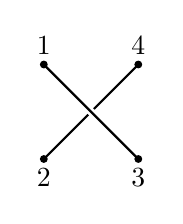
\begin{tikzpicture}[scale=.6]
            \draw[black,thick] (-1,-1) -- (-.06,-.06);
            \draw[black,thick] (.06,.06) -- (1,1);
            \draw[black,thick] (-1,1) -- (1,-1);
            \filldraw[black] (-1,-1) circle (2pt) node[anchor=north] {2};
            \filldraw[black] (-1,1) circle (2pt) node[anchor=south] {1};
            \filldraw[black] (1,-1) circle (2pt) node[anchor=north] {3};
            \filldraw[black] (1,1) circle (2pt) node[anchor=south] {4};
        \end{tikzpicture}
        
        一个tikz示意图
    \end{center}
}

本模板支持在特定页面取消margin,重新设置当前页面的布局,只需使用本模板提供的
\verb|\nomargin|命令即可。

同时本模板支持两种布局格式:
\begin{itemize}
    \item 带有margin的默认模式,margin的宽为1.5cm,位于页面的右侧,当然本模板仍提供了没有margin的\verb|nomarg|环境
    \item 取消margin的普通布局,需使用\verb|\nomargin|开启,使用\verb|\margin|结束,
        两者之间的内容为取消margin之后的页面布局,并且自动换页。如果忘记使用\verb|\margin|命令结尾的话,
        后续的页面布局中布局会乱排。
\end{itemize}

所以一定要养成良好习惯,前后命令成对书写\footnote[1]{注意:没有nomargin对应的局部环境}

\vfill 

\textcolor{red}{\thepage{}页底部}


% 使用\nomargin后会自动换页
\nomargin
\subsection{Margin测试}
使用\verb|\nomargin|后会自动换页,比如从这里的第\number\numexpr\value{page}-1页自动换到\thepage{}页:
\begin{verbatim}
    % 第一页内容 ...
    \nomargin
    \section{Margin测试}
    使用\verb|\nomargin|后会自动换页,...

    \section{脚注测试}
    本模板还对footnote进行了相关的定制,...
    \begin{itemize}
        \item footnote定制\footnote[1]{这是第一个脚注}
        \item footnote定制\footnote[2]{这是第二个脚注}
    \end{itemize}
    \margin
\end{verbatim}

还有就是可以从下面的公式布局看出当前是否有margin,
\begin{align}
    \sum_{i=1}^{+\infty}{\int_{0}^{i}-\frac{1}{t}\mathrm{d}t} = \frac{\pi^2}{6}
\end{align}


\subsection{脚注测试}
本模板还对footnote进行了相关的定制,使用\verb|\footnote|命令,会自动将脚注编号添加到脚注内容上。设置了
footskip等值,使用效果如下:
\begin{itemize}
    \item footnote定制\footnote[1]{这是第一个脚注}
    \item footnote定制\footnote[2]{这是第二个脚注}
\end{itemize}
\vfill 

\textcolor{red}{\thepage{}页底部}
\margin




\section{正文环境}
由于本模板的简洁特性,于是相应的正文环境也进行了相应的简化,没有 
什么光彩夺目的文本环境。但是你可以把marginnote和footnote看作
一种环境


\section{数学环境}
本模板定义了如下的数学环境,都是相较于简洁的,符合整个模板的灰色主题。具体每一个环境的使用方法和
效果,请参见如下的示例:

\subsection{定义环境}
\begin{bytes}[10]
\begin{definition}[Euler Formula]
    测试如下著名的Euler公式, Take the famous Euler's Formula As Example:
    \begin{align}
        \sum_{i=1}^{+\infty}{\int_{0}^{i}-\frac{1}{t}\mathrm{d}t} = \frac{\pi^2}{6}
    \end{align}
\end{definition}
\end{bytes}
\begin{definition}[Euler Formula]
测试如下著名的Euler公式, Take the famous Euler's Formula As Example:
\begin{align}
    \sum_{i=1}^{+\infty}{\int_{0}^{i}-\frac{1}{t}\mathrm{d}t} = \frac{\pi^2}{6}
\end{align}
\end{definition}

\marginnote{定义与定理环境可能在后期会进行合并,或单独的更改}

\subsection{定理环境}
\begin{bytes}[10]
\begin{theorem}
    含有一阶导函数的泛函定义如下:
    \begin{align}
        \begin{aligned}
            \delta F
            & = F[x,U+\delta U,U'+\delta U']-F[x,U,U']  \\
            & = \left[\frac{\partial F}{\partial U}\delta U+\frac{\partial F}{\partial U'}\delta U'\right]+\frac{\partial^2F}{\partial U\partial U'}\delta U\delta U'+\frac{1}{2!}\left[\frac{\partial^2F}{\partial U^2}\delta U^2+\frac{\partial^2F}{\partial U'^2}\delta U'^2\right]+\cdots \\
            & = ...
        \end{aligned}
    \end{align}
\end{theorem}
\end{bytes}
\begin{theorem}
含有一阶导函数的泛函定义如下:
\begin{align}
    \begin{aligned}
        \delta F
        & = F[x,U+\delta U,U'+\delta U']-F[x,U,U']  \\
        & = \left[\frac{\partial F}{\partial U}\delta U+\frac{\partial F}{\partial U'}\delta U'\right]+\frac{\partial^2F}{\partial U\partial U'}\delta U\delta U'+\frac{1}{2!}\left[\frac{\partial^2F}{\partial U^2}\delta U^2+\frac{\partial^2F}{\partial U'^2}\delta U'^2\right]+\cdots \\
        & =\varepsilon\left[\frac{\partial F}{\partial U}\eta+\frac{\partial F}{\partial U'}\eta^{\prime}\right]+\frac{\varepsilon^{2}}{2}\left[\cdots\right.
    \end{aligned}
\end{align}
\end{theorem}

\subsection{命题环境}
\begin{bytes}[10]
\begin{proposition}[某命题]
    这是一个命题环境, this is a proposition env
\end{proposition}
\end{bytes}
\begin{proposition}[某命题]
    这是一个命题环境, this is a proposition env
\end{proposition}

\marginnote{这部分的内容可能也会在后期有着较大的变动}

\subsection{推论环境}
\begin{bytes}[10]
\begin{corollary}[某推论]
    这是一个推论环境, this is a corollary env
\end{corollary}
\end{bytes}
\begin{corollary}[某推论]
    这是一个推论环境, this is a corollary env
\end{corollary}

\subsection{引理环境}
\begin{bytes}[10]
\begin{lemma}[某引理]
    这是一个引理环境, this is a lemma env
\end{lemma}
\end{bytes}
\begin{lemma}[某引理]
    这是一个引理环境, this is a lemma env
\end{lemma}





\clearpage
\subsection{抄录环境}
本模板提供了部分代码抄录环境 \verb|bytes, code|,抄录环境\verb|code|使用\verb|\lstset|命令进行设置,
比如下面指定编程语言的高亮选择,这里以Python举例.\footnote[2]{lislisting已经定义了几十种语言的高亮,详情请参见lislisting的2.4.1小节}

\begin{code}{python}
for circle_index in range(CIRCLE_NUM):
    coors_set_pure = np.array([item for item in coors_set[circle_index, :] if item is not None and point_is_in(item)])
    point_amount += coors_set_pure.size/2
    if coors_set_pure.size == 0:
        continue
    # 把有效坐标保存
    if circle_index == 0:
        all_coors = pd.DataFrame(coors_set_pure)
\end{code}

\begin{code}{C}
int main() {
    int data[] = {8, 7, 2, 1, 0, 9, 6};
    int n = sizeof(data) / sizeof(data[0]);
    printf("Original array: \n");
    for (int i = 0; i < n; i++) {
        printf("%d ", data[i]);
    }
    printf("\n");
    
    quickSort(data, 0, n - 1);
    
    printf("Sorted array: \n");
    for (int i = 0; i < n; i++) {
        printf("%d ", data[i]);
    }
    return 0;
}    
\end{code}
\marginnote[-23em]{注意:这里的语言类型C/C++需要大写,不然会报错}

当然我们也可以不指定编程语言的类别,直接原样输出:
\begin{bytes}
\newcounter{definition}
\newenvironment{definition}[1][]{%   
        \stepcounter{definition}%
        \begin{tcolorbox}[%
            enhanced,
            arc=3pt,
            frame hidden,
            % suppressfootnotes=true,
}{\end{tcolorbox}}
\end{bytes}


\vfill
\textcolor{red}{\kaishu 关于footnote还有一个bug:如果height没有填满,那么footnote就不会到最底部}

\section{图形绘制}
在开发本文档类 \zlatex{}时,我也同时开发了对应的绘图宏包。
往往来说,新手认为在\TeX{}中绘制图形是一件很麻烦的事情,即便是
经常用\LaTeX{}的朋友,在绘制一些简单的图形时,也会觉得比较麻烦。
但是在\TeX{}中绘图,麻烦的还不知语法的本身,更重要的是引入 \verb|tikz|
这中大型宏包之后,本身的编译速度就会变得十分的缓慢,于是本模板开率开发其他的宏包
用于调用外部函数进行绘图,减少文档的编译时长。

\zlatex{}宏包中内置了\texttt{FunctionPlot}宏包,其作用就是用来绘制各种图像,
包括普通形状绘制,2维函数绘制,3维函数绘制。自己在之前的命令基础上又重新定义了两个使用
gnuplot的绘图命令,这样可以使得编译速度进一步加快。同时也对图形设置了默认的选项,免去了
读者去翻阅官方文档的麻烦。

\subsection{基本图形绘制}
其中就包含基础的圆,三角形,直角三角形,平行四边形,梯形,平行线,
以及各种基本图形。
对应的命令调用格式如下:
\begin{bytes}
% 1.圆
\circle[center]{radius}
% 2.三角形
\triangle[center]{side}
% 3.矩形
\rectangle[center][width][angle]{height}
\end{bytes}


% \clearpage
\subsection{函数绘制}
函数的绘制类型是十分的丰富的,包括:
\marginnote{注意:这里只列出了部分图形绘制类型,完整列表请参考官方文档。对应的tikz指令也可以用户自定义}

\begin{framed}
\begin{multicols}{3}
    \begin{itemize}    
        \item 显式函数
            \begin{itemize}
                \item 二维函数
                \item 3维函数
                \item 参数方程
                \item 数据绘图
            \end{itemize}
        \item 隐式函数
        \begin{itemize}
            \item 2维函数
            \item 3维函数
            \item 参数方程
            \item 数据绘图
        \end{itemize} 
        \item 外部程序
        \begin{itemize}
            \item gnuplot 
            \item mathematica
            \item matlab
            \item python
        \end{itemize} 
\end{itemize} 
\end{multicols}
\end{framed}


\newcommand{\Note}[1]{\texttt{#1}}
至于普通的二三维的函数绘图十分简单的,你可以指定一下绘制的颜色,
或者说是colormap,定义域之类的plot parameters,尽情发挥。
下面我们主要绘制了 $y=x\sin(2x)$, $z=x*y$两个函数,效果还是可以的。

\nomargin
% \Gplot[scale]{color}{f(x)}
\begin{center}
    \Gplot[1.2]{blue, domain=-12:12}{x*sin(2*x)}
    \Gplotz[.08]{bluered}{x*y}   

    \Gplotz[.1]{cool}{x*y}
\end{center}

\subsection{参数方程绘图}
主要是在vscode中定义了下面5个绘制命令的trigger
\begin{lstlisting}
trigger    --> 展开式
plot2d     --> \Gplot[scale]{color}{f(x)}
plot3d     --> \Gplotz[scale]{colormap style}{f(x, y)}
polarplot  --> \polarplot[scale][plot parameters]{f(\t)}
paraplot2d --> \paraplot[scale][plot parameters]{{x(t)},{y(t)}}
paraplot3d --> \paraplotz[scale][plot parameters]{{x(t)},{y(t)}}
\end{lstlisting}

其实参数方程作图主要就是\Note{极坐标},\Note{二维参数方程},
\Note{三维参数方程}这三种常见的情形.


那么我们就首先绘制极坐标的图形,下面我们绘制图形对应的方程分别为:
\begin{align}
    & \rho = \frac{0.01}{\pi \theta}\\
    & \rho = \sin(\theta)
\end{align}
\margin

\marginnote[2em]{只需要注意的一个点:paraplot默认使用的是角度,而非弧度}

\begin{center}
    \polarplot[.7][red, domain=0:1440]{0.01/pi*\t}
    \polarplot[2][blue,thick,domain=0:120]{sin(\t)}
\end{center}


既然极坐标我们能够画出来了,那么接下来就是参数方程了,
\begin{center}
    \paraplot{{3*cos(t)}, {sin(t)}}
    \paraplot[.75][domain=1:2, orange, very thick]{{t}, {-2.5*(t-1.5)^2}}
\end{center}

最后就是我们的三维参数方程了,气质也是和上面的二维方程一样的,因为我们默认
$z(t) = t$,演示效果如下:下面我们绘制了螺旋线的方程 $x=\sin(t),y=3*\cos(t)(y=\cos(t)),z=t$
\begin{center}
    \paraplotz[.8]{{sin(t)}, {3*cos(t)}}
    \paraplotz[.8][blue,very thick,domain=0:1440]{{sin(t)}, {cos(t)}}
\end{center}

同理,对应的MMA模块我也归纳到了FunctionPlot宏包中,
用于调用MMA生成对应的pdf矢量图片

\subsection{计算}
\begin{align}
    \wolfram{Series[Exp[x], {x, 0, 5}]}
\end{align}

\subsection{图片插入}
MMA 图片测试,下面的这个绘图还是比较复杂的,于是我们使用MMA绘制。

\begin{figure}[!htb]
    \centering
    \wolframgraphics{
		ContourPlot[
		x^2/4 + y^2/3 == 5, {x, -5, 5}, {y, -5, 5},
		ContourStyle->{
			% 同样的,被latex注释的部分不会传入MMA
			% RGBColor["\#00C0A3"], 
			% 在传参的过程中,不要使用#,即使是\#,MMA也是会报错的。
			RGBColor[0.,0.7529411764705882,0.6392156862745098],
			Thickness[0.004]
		},
		AspectRatio->1, 
		AxesOrigin->{0,0}, 
		Axes->True,
		Frame->False,
		AxesStyle->Arrowheads[{0, 0.03}],
		AxesLabel->{"x", "y"}
	]}{MMA2d1}
    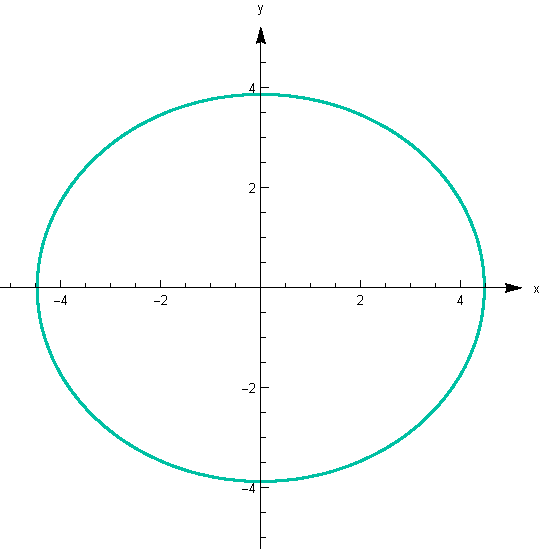
\includegraphics[scale=.7]{MMA2d1.pdf}
	\caption{MMA 二维图形}
	\label{MMA 二维图形}
\end{figure}

\begin{figure}[!htb]
    \centering
    \wolframgraphics{
    NumberLinePlot[
	    {Interval[{5, Infinity}], Interval[{2, 7}]}, 
	    AxesStyle->Arrowheads[{0, 0.03}]
    ]
    }{MMA2d2}
    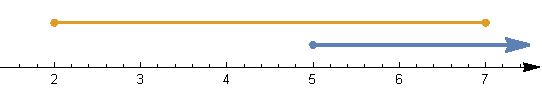
\includegraphics[scale=.7]{MMA2d2.pdf}
    \caption{MMA 二维图形2}
    \label{MMA 二维图形2}
\end{figure}

二维的一些图形绘制了之后,自然要去绘制一些MMA中的3维对象了。下面就是
一些例子:

\begin{figure}[!htb]
    \centering
    \wolframgraphics{
        Arrow[Tube[
		    BSplineCurve[{{0,0,0}, {.2,1,0.5},{2,1,1}}]
        ]]//Graphics3D}{MMA3d1}
    \wolframgraphics{
        VectorPlot3D[
            {x, y, z}, {x, -1, 1}, 
            {y, -1, 1}, {z,-1, 1},
            PlotTheme->"Classic"
        ]}{MMA3d2}
    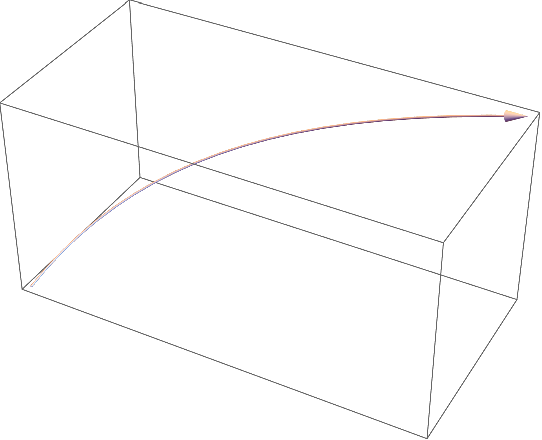
\includegraphics[scale=.7]{MMA3d1.pdf}
    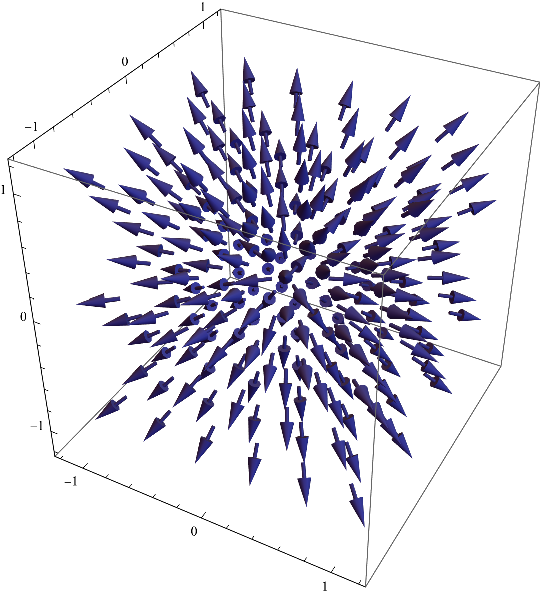
\includegraphics[scale=.7]{MMA3d2.pdf}
    \caption{MMA 三维图形}
    \label{MMA 三维图形}
\end{figure}


\subsection{表格功能}
MMA还能够解方程,微分方程,求根公式,输出表格等等.




\chapter{\zlatex{} Insight}
\section{设计流程}
本模板的设计流程大致如下:
\begin{itemize}
    \item 首先确定自己的页面布局,因为我这个模板是希望能够用于记笔记的,
        并且希望有margin,于是就选择了一个较宽的页面布局,这就是为什么和其他的模板不同
    \item 在确定自己的基本页面尺寸后便可以考虑另一个比较大的方面:页脚,页眉,本模板采用的是\verb|fancyhdr|宏包
    \item 然后是这个模板的语言,一般来说大部分人都是自用,也就没有去考虑英文,在这里我想说的是,你得有这种意识
        让你的模板能够有更多得适应面,也可以提高你使用 \TeX{}的能力
    \item 接下来是正文部分,在正文部分你首先应该考虑你需要使用的计数器(文章结构),需要chapter吗? 需要part吗?
        确定层级顺序后便可以着手设计你的目录,本模板使用的是 \verb|tocloft|宏包
    \item 接下来应该才是大部分人关心的部分,什么数学环境,代码环境,表格,图片等
\end{itemize}

\section{设计原则}
\subsection{简洁}
本模板没有花里胡哨的各种设计元素,主题颜色偏向灰色,没有很多的色彩,如果
使用者想要更加多彩设计元素可以使用\verb|ElegantLaTeX|系列模板.

简洁也就意味着本模板没有使用过多宏包,大部分命令均是通过 \LaTeX2$\varepsilon{}$ 的一些
primitive定义,甚至部分结构的达成是通过 \TeX{}的primitive完成。这样的一个好处就是,
本模板的使用者可以在此模板基础上自由的接入其他宏包,而不必考虑宏包的冲突问题。


\subsection{编译速度}
由于大部分人均是使用的windows,只要你的文章稍微多一些,速度就下去了。于是本模板充分
考虑到\LaTeX{}中各个耗时的宏包,代码块,编译引擎差异。在tikz绘图和数值计算方面均采用
外部程序完成,这样可以一定程度上增加编译速度。


\subsection{自定义}
在这一章节我会深入的介绍本模板的工作方式,以及其中定义的命令.比如我们这里对content进行了重写:
\marginnote{这里自定义命令大部分基于\LaTeX2$\varepsilon{}$}[-12em]

\begin{verbatim}
    %% 1.原始自定义命令
    \raise\the\dimexpr-\ch@pterskip-\title@skip%
        \hbox{\rule{.03\textwidth}{.006\textheight}}\kern-1em%
    \raise\the\dimexpr-\ch@pterskip-\title@skip%
        \hbox{\rule{\dimexpr.95\textwidth-1em}{.5pt}}
    \raise\the\dimexpr\ch@pterskip-2em\hbox{\vspace*{\the\ch@pterskip}}%
    \kern-1em\large Chapter \Roman{chapter}: #1
\end{verbatim}


同时考虑到overfull hbox,改进了原始的命令,改进后的命令如下,此时我们便已经修复了原始contents中的
overfull hbox问题:
\begin{verbatim}
    % 使用新的chapter命令
    \let\old@chapter\chapter
    \renewcommand{\chapter}[1]{%
        \ifnum\value{chapter}=1\relax
            \setlength{\title@skip}{-4em}
        \else%
            \setlength{\title@skip}{0em}
        \fi
        \addtocontents{toc}{%
            \protect\mbox{}\protect\hspace*{1.7em}%
                \rule[\the\title@skip]{.03\textwidth}{.006\textheight}%
            \rule[\the\title@skip]{\dimexpr.96\textwidth-2em}{.5pt}\par%
        }
        \old@chapter{#1}
    }
\end{verbatim}


\chapter{我与\TeX{}}
\section{回忆}
我为什么用\TeX{}? \TeX{}带给了我什么?

\subsection{为什么是\TeX{}?}
究竟什么是 \TeX{}??

\subsection{为什么要用\TeX{}?}



\chapter{致谢}
\section{致谢}
\subsection{模板参考}
本模板参考了如下的优秀模板:
\begin{itemize}
    \item Beautiful\LaTeX{}
    \item Elegant\LaTeX{}
    \item Notes\TeX{} V3
    \item Memoir
    \item CUMCMThesis
\end{itemize}

\subsection{文档参考}



\section{结语}
望诸君皆能找到自己之所爱.


\end{document}

